%Este trabalho está licenciado sob a Licença Creative Commons Atribuição-CompartilhaIgual 3.0 Não Adaptada. Para ver uma cópia desta licença, visite http://creativecommons.org/licenses/by-sa/3.0/ ou envie uma carta para Creative Commons, PO Box 1866, Mountain View, CA 94042, USA.

%\documentclass[main.tex]{subfiles}
%\begin{document}

\chapter{Solução de sistemas lineares}\index{sistema linear}

Neste parte de nosso curso, estamos interessados em técnicas para resolução de sistemas de equações algébricas lineares. 

Trataremos de sistemas de equações algébricas lineares da seguinte forma:
\begin{eqnarray*}
a_{11}x_1 + a_{12}x_2 + \cdots +a_{1n}x_n &=& y_1\\
a_{21}x_1 + a_{22}x_2 + \cdots +a_{2n}x_n &=& y_2\\
 &\vdots &\\
a_{m1}x_1 + a_{m2}x_2 + \cdots +a_{mn}x_n &=& y_m\\
\end{eqnarray*}
Observe que $m$ é o número de equações e $n$ é o número de incógnitas.  Podemos escrever este problema na forma matricial
$$Ax=y$$
onde
$$A=\left[\begin{array}{cccc}
a_{11} & a_{12} & \cdots & a_{1n}\\
a_{21} & a_{22} & \cdots & a_{2n}\\
\vdots & \vdots & \ddots & \vdots\\
a_{m1} & a_{m2} & \cdots & a_{mn}
\end{array}
\right]~~~x=\left[\begin{array}{c}
x_{1} \\
x_{2} \\
\vdots \\
x_{n}
\end{array}
\right]~~~y=\left[\begin{array}{c}
y_{1} \\
y_{2} \\
\vdots \\
y_{m}
\end{array}
\right]$$

Daremos mais atenção ao caso $m=n$, isto é, quando a matriz $A$ que envolvia no sistema linear é quadrada.


\section{Eliminação gaussiana com pivoteamento parcial}\index{eliminação gaussiana!com pivoteamento parcial}
Lembramos que algumas operações feitas nas linhas de um sistema não alteram a solução:
\begin{enumerate}
\item Multiplicação de um linha por um número
\item Troca de uma linha por ela mesma somada a um múltiplo de outra.
\item Troca de duas linhas.
\end{enumerate}

O processo que transforma um sistema em outro com mesma solução, mas que apresenta uma forma triangular é chamado eliminação Gaussiana. A solução do sistema pode ser obtida fazendo substituição regressiva.
\begin{ex}[Eliminação Gaussiana sem pivotamento parcial] Resolva o sistema:
  \begin{equation*}
    \left\{\begin{array}{c}
        x+y+z=1\\
        2x+y-z=0\\
        2x+2y+z=1
      \end{array}\right.  
  \end{equation*}
\end{ex}
\begin{sol}
Escrevemos a matriz completa do sistema:
\begin{equation*}
  \left[\begin{array}{ccc|c}
      1 &1& 1&1\\
      2 &1& -1&0\\
      2 & 2 &1&1
    \end{array}\right] \sim 
  \left[\begin{array}{ccc|c}
      1 &1& 1&1\\
      0 &-1& -3&-2\\
      0 & 0 &-1&-1
    \end{array}\right]
\end{equation*}
Encontramos $-z=-1$, ou seja, $z=1$. Substituímos na segunda equação e temos $-y-3z=-2$, ou seja, $y=-1$ e, finalmente $x+y+z=1$, resultando em $x=1$.
\end{sol}

A Eliminação Gaussiana com pivotamento parcial consiste em fazer uma permutação de linhas de forma a escolher o maior pivô (em módulo) a cada passo.

\begin{ex}[Eliminação Gaussiana com pivotamento parcial] Resolva o sistema:
$$\left\{
\begin{array}{c}
x+y+z=1\\
2x+y-z=0\\
2x+2z+z=1
\end{array}\right.
$$
\end{ex}
\begin{sol}
Escrevemos a matriz completa do sistema:
\begin{eqnarray*}\left[
\begin{array}{ccc|c}
1 &1& 1&1\\
2 &1& -1&0\\
2 & 2 &1&1
\end{array}
\right] &\sim& \left[
\begin{array}{ccc|c}
2 &1& -1&0\\
1 &1& 1&1\\
2 & 2 &1&1
\end{array}
\right] \\ & \sim & \left[
\begin{array}{ccc|c}
2 &1& -1&0\\
0 &1/2& 3/2&1\\
0 & 1 &2&1
\end{array}
\right]\\ & \sim & \left[
\begin{array}{ccc|c}
2 &1& -1&0\\
0 & 1 &2&1\\
0 &1/2& 3/2&1
\end{array}
\right]\\ & \sim & \left[
\begin{array}{ccc|c}
2 &1& -1&0\\
0 & 1 &2&1\\
0 &0& 1/2&1/2
\end{array}
\right]
\end{eqnarray*}
Encontramos $1/2z=1/2$, ou seja, $z=1$. Substituímos na segunda equação e temos $y+2z=1$, ou seja, $y=-1$ e, finalmente $2x+y-z=0$, resultando em $x=1$.
\end{sol}

\begin{ex}
Resolva o seguinte sistema por eliminação gaussiana com pivotamento parcial.
\begin{equation*}
\left[
\begin{array}{ccc}
0 &2& 2\\
1 &2& 1\\
1 & 1 &1
\end{array}
\right]
\left[
\begin{array}{c}
x\\
y\\
z
\end{array}
\right]=
\left[
\begin{array}{c}
8\\
9\\
6
\end{array}
\right]  
\end{equation*}
\end{ex}
\begin{sol}
Construímos a matriz completa:
\begin{eqnarray*}\left[
\begin{array}{ccc|c}
0 &2& 2&8\\
1 &2& 1&9\\
1 & 1 &1&6
\end{array}
\right] &\sim&
\left[
\begin{array}{ccc|c}
1 &2& 1&9\\
0 &2& 2&8\\
1 & 1 &1&6
\end{array}
\right] \\ 
&\sim&
\left[
\begin{array}{ccc|c}
1 &2& 1&9\\
0 &2& 2&8\\
0 & -1 &0&-3
\end{array}
\right]\\
&\sim&
\left[
\begin{array}{ccc|c}
1 &2& 1&9\\
0 &2& 2&8\\
0 & 0 &1&1
\end{array}
\right]\\
&\sim&
\left[
\begin{array}{ccc|c}
1 &2& 0&8\\
0 &2& 0&6\\
0 & 0 &1&1
\end{array}
\right]\\
&\sim&
\left[
\begin{array}{ccc|c}
1 &0& 0&2\\
0 &2& 0&6\\
0 & 0 &1&1
\end{array}
\right]
\end{eqnarray*}
Portanto $x=2$, $y=3$ e $z=1$.
\end{sol}

\begin{ex}[Problema com elementos com grande diferença de escala]
$$\left[\begin{array}{cc}
\varepsilon & 2\\
1 & \varepsilon
\end{array}\right]
\left[\begin{array}{c}x\\y
\end{array}\right]=
\left[\begin{array}{c}4\\3
\end{array}\right]
$$
Executamos a eliminação gaussiana sem pivotamento parcial para $\varepsilon \neq 0$ e $|\varepsilon|<<1$:
$$\left[\begin{array}{cc|c}
\varepsilon & 2 & 4\\
1 & \varepsilon & 3
\end{array}
\right]\sim\left[\begin{array}{cc|c}
\varepsilon & 2 & 4\\
0 & \varepsilon-\frac{2}{\varepsilon} & 3-\frac{4}{\varepsilon}
\end{array}
\right]
%\sim
%\left[\begin{array}{cc|c}
%\varepsilon & 0 & 4-\left(3-\frac{4}{\varepsilon}\right) \frac{2}{\varepsilon-\frac{2}{\varepsilon}}\\
%0 & \varepsilon-\frac{2}{\varepsilon} & 3-\frac{4}{\varepsilon}
%\end{array}
%\right]
$$

Temos
$$y=\frac{3-4/\varepsilon}{\varepsilon-2/\varepsilon}$$%=2-{\frac {3}{2}}\varepsilon+{\varepsilon}^{2}-{\frac {3}{4}}{\varepsilon}^{3}+{\frac {1}{2}}{\varepsilon}^{4}+O(\varepsilon^5)$$
e
$$x=\frac{4-2y}{\varepsilon}$$ %3-2\varepsilon+{\frac {3}{2}}{\varepsilon}^{2}-{\varepsilon}^{3}+{\frac {3}{4}}{\varepsilon}^{4}+O(\varepsilon^5)$$

Observe que a expressão obtida para  $y$ se aproximada de $2$ quando $\varepsilon$ é pequeno:
$$y=\frac{3-4/\varepsilon}{\varepsilon-2/\varepsilon}=\frac{3\varepsilon-4}{\varepsilon^2-2} \longrightarrow \frac{-4}{-2}=2, ~~\hbox{quando}~\varepsilon \to 0.$$
Já expressão obtida para $x$ depende justamente da diferença $2-y$:
$$x=\frac{4-2y}{\varepsilon}=\frac{2}{\varepsilon} (2-y)$$

Assim, quando $\varepsilon$ é pequeno, a primeira expressão, implementado em um sistema de ponto flutuante de acurácia finita, produz $y= 2$ e, consequentemente, a expressão para $x$ produz $x=0$. Isto é, estamos diante um problema de cancelamento catastrófico.

Agora, quando usamos a Eliminação Gaussiana com pivotamento parcial, fazemos uma permutação de linhas de forma a escolher o maior pivô a cada passo:

$$\left[\begin{array}{cc|c}
\varepsilon & 2 & 4\\
1 & \varepsilon & 3
\end{array}
\right]\sim
\left[\begin{array}{cc|c}
1 & \varepsilon & 3\\
\varepsilon & 2 & 4
\end{array}
\right]\sim
\left[\begin{array}{cc|c}
1 & \varepsilon & 3\\
0 & 2-\varepsilon^2 & 4-3\varepsilon
\end{array}
\right]
$$

Continuando o procedimento, temos:
$$y=\frac{4-4\varepsilon}{2-\varepsilon^2}$$ e
$$x=3-\varepsilon y$$
\end{ex}

Observe que tais expressões são analiticamente idênticas às anteriores, no entanto, são mais estáveis numericamente. Quando $\varepsilon$ converge a zero, $y$ converge a $2$, como no caso anterior. No entanto, mesmo que $y=2$, a segunda expressão produz $x=3-\varepsilon y$, isto é, a aproximação $x\approx 3$ não depende mais de obter $2-y$ com precisão.

\section*{Exercícios}

\begin{Exercise}\label{prob_gausspp} Resolva o seguinte sistema de equações lineares
\begin{eqnarray*}
x+y+z&=&0\\
x+10z&=&-48\\
10y+z&=&25
\end{eqnarray*} Usando eliminação gaussiana com pivoteamento parcial (não use o computador para resolver essa questão).
\end{Exercise}
\begin{Answer}
  \begin{tiny}
Escrevemos o sistema na forma matricial e resolvemos:
\begin{eqnarray*}
\left[
\begin{array}{ccc|c}
1&1&1&0\\
1&0&10&-48\\
0&10&1&25
\end{array}\right] &\sim&
\left[
\begin{array}{ccc|c}
1&1&1&0\\
0&-1&9&-48\\
0&10&1&25
\end{array}\right] \sim
\left[
\begin{array}{ccc|c}
1&1&1&0\\
0&10&1&25\\
0&-1&9&-48
\end{array}\right]\sim\\
&\sim&\left[
\begin{array}{ccc|c}
1&1&1&0\\
0&10&1&25\\
0&0&9.1&-45.5
\end{array}\right]\sim
\left[
\begin{array}{ccc|c}
1&1&1&0\\
0&10&1&25\\
0&0&1&-5
\end{array}\right]\sim\\
&\sim&\left[
\begin{array}{ccc|c}
1&1&0&5\\
0&10&0&30\\
0&0&1&-5
\end{array}\right]
\sim\left[
\begin{array}{ccc|c}
1&1&0&5\\
0&1&0&3\\
0&0&1&-5
\end{array}\right]\sim\\
&\sim&\left[
\begin{array}{ccc|c}
1&0&0&2\\
0&1&0&3\\
0&0&1&-5
\end{array}\right]
\end{eqnarray*}
Portanto $x=2$, $y=3$, $z=-5$
      \end{tiny}
\end{Answer}

\begin{Exercise} Resolva o seguinte sistema de equações lineares
\begin{eqnarray*}
x+y+z&=&0\\
x+10z&=&-48\\
10y+z&=&25
\end{eqnarray*} Usando eliminação gaussiana com pivotamento parcial (não use o computador para resolver essa questão).
\end{Exercise}

\begin{Exercise}Calcule a inversa da matriz
$$
A=\left[\begin{array}{ccc}
1&2&-1\\
-1&2&0\\
2&1&-1
\end{array}
\right]
$$
usando eliminação Gaussiana com pivotamento parcial.
\end{Exercise}

\begin{Exercise} \label{inv22} Demonstre que se $ad\neq bc$, então a matriz $A$ dada por:
$$A=\left[\begin{array}{cc}a&b\\c&d\end{array}\right]$$
é inversível e sua inversa é dada por:
$$A^{-1}= \frac{1}{ad-bc} \left[\begin{array}{cc}d&-b\\-c&a\end{array}\right].$$
\end{Exercise}

\ifisscilab
\begin{Exercise} Considere as matrizes
$$A=
\left[
\begin{array}{ccc}
0&0&1\\
0&1&0\\
1&0&0
\end{array}\right]$$
e
$$E=
\left[
\begin{array}{ccc}
1&1&1\\
1&1&1\\
1&1&1
\end{array}\right]$$
e o vetor
$$v=
\left[
\begin{array}{c}
2\\
3\\
4
\end{array}\right]$$
\begin{itemize}
\item[a)] Resolva o sistema $Ax=v$ sem usar o computador.
\item[b)] Sem usar o computador e através da técnica algébrica de sua preferência, resolva o sistema $(A+\varepsilon E)x_\varepsilon=v$ considerando $|\varepsilon|<<1$ e obtenha a solução exata em função do parâmetro $\varepsilon$.
\item[c)] Usando a expressão analítica obtida acima, calcule o limite $\lim_{\varepsilon\to 0} x_\varepsilon $.
\item[d)] Resolva o sistema $(A+\varepsilon E)x=v$ no \verb+Scilab+ usando pivotamento parcial e depois sem usar pivotamento parcial para valores muito pequenos de $\varepsilon$ como $10^{-10}, 10^{-15}, \ldots$. O que você observa?
\end{itemize}
\end{Exercise}
\begin{Answer}
  \begin{tiny}
\begin{itemize}
\item[a)] $x=[4 ~~3 ~~2]^T$

\item[b)] O sistema é equivalente a
$$
\begin{array}{lclclcl}
\varepsilon x_1 &+& \varepsilon x_2 &+&(1+\varepsilon) x_3 &=& 2\\
\varepsilon x_1 &+& (1+\varepsilon) x_2 &+&\varepsilon x_3 &=& 3\\
(1+\varepsilon) x_1 &+& \varepsilon x_2 &+&\varepsilon x_3 &=& 4\\
\end{array}
$$
Somando as três equações temos
$$(1+3\varepsilon)(x_1+x_2+x_3)=9\Longrightarrow x_1+x_2+x_3=\frac{9}{1+3\varepsilon}$$
Subtraímos $\varepsilon(x_1+x_2+x_3)$ da cada equação do sistema original e temos:
$$\begin{array}{l}
x_3=2-\frac{9\varepsilon}{1+3\varepsilon}\\[.4cm]
x_2=3-\frac{9\varepsilon}{1+3\varepsilon}\\[.4cm]
x_1=4-\frac{9\varepsilon}{1+3\varepsilon}
\end{array}
$$
Assim temos:
$$x_{\varepsilon}=\left[4 ~~3 ~~2\right]^T-\frac{9\varepsilon}{1+3\varepsilon}\left[1 ~~1 ~~1\right]^T$$
\end{itemize}
      \end{tiny}
\end{Answer}
\fi

\ifisscilab
\begin{Exercise}\label{trid} Resolva o seguinte sistema de $5$ equações lineares
\begin{eqnarray*}
x_1-x_2&=&0\\
-x_{i-1}+2.5x_i-x_{i+1}&=&e^{-\frac{(i-3)^2}{20}},\qquad 2\leq i \leq 4\\
2x_{5}-x_{4}&=&0
\end{eqnarray*}
representando-o como um problema do tipo $Ax=b$ no \verb+Scilab+ e usando o comando de contra-barra para resolvê-lo. Repita usando a rotina que implementa eliminação gaussiana.
\end{Exercise}
\begin{Answer}
  \begin{tiny}
 $x=[ 1.6890368  ~~  1.6890368  ~~  1.5823257  ~~  1.2667776   ~~ 0.6333888]^{T}$    
  \end{tiny}
\end{Answer}
\fi

\ifisscilab
\begin{Exercise} Encontre a inversa da matriz
$$\left[
\begin{array}{ccc}
1&1&1\\
1&-1&2\\
1&1&4
\end{array}\right]$$
\begin{itemize}
\item[a)] Usando Eliminação Gaussiana com pivotamento parcial à mão.
\item[b)] Usando a rotina 'gausspp()'.
\item[c)] Usando a rotina 'inv()' do \verb+Scilab+.
\end{itemize}
\end{Exercise}
\begin{Answer}
  \begin{tiny}
 $$ \left[ \begin {array}{ccc} 1&1/2&-1/2\\1/3&-1/2&1/6
\\-1/3&0&1/3\end {array} \right] $$    
  \end{tiny}
\end{Answer}
\fi

\section{Condicionamento de sistemas lineares}\index{sistema linear!condicionamento}\index{matriz!condicionamento}

Quando lidamos com matrizes no corpo do números reais (ou complexos), existem apenas duas alternativas: i) a matriz é inversível; ii) a matriz não é inversível e, neste caso, é chamada de matriz singular. Ao lidarmos em aritmética de precisão finita, encontramos uma situação mais sutil: alguns problema lineares são mais difíceis de serem resolvidos, pois os erros de arredondamento se propagam de forma mais significativa que em outros problemas. Neste caso falamos de problemas bem-condicionados e mal-condicionados. Intuitivamente falando, um problema bem-condicionado é um problema em que os erros de arredondamento se propagam de forma menos importante; enquanto problemas mal-condicionados são problemas em que os erros se propagam de forma mais relevante.

Um caso típico de sistema mal-condicionado é aquele cujos coeficiente estão muito próximos ao de um problema singular. Considere o seguinte exemplo:

\begin{ex} Observe que o problema
$$\left\{ \begin{array}{l}71x+41y=100\\
\lambda x+30y=70
\end{array}
\right.$$
é impossível quando $\lambda= \frac{71\times 30}{41}\approx 51,95122$.

Agora, verifique o que acontece quando resolvemos os seguintes sistemas lineares:
$$\left\{ \begin{array}{l}71x+41y=100\\
52x+30y=70
\end{array}
\right. \\ \hbox{ e }
\left\{ \begin{array}{l}71x+41y=100\\
51x+30y=70
\end{array}
\right. \\
$$
A solução do primeiro problema é $x=-65$ e $y=115$. Já para o segundo problema é $x=\frac{10}{3}$ e $y=-\frac{10}{3}$.

Igualmente, observe os seguintes dois problemas:
$$\left\{ \begin{array}{l}71x+41y=100\\
52x+30y=70
\end{array}
\right. \\ \hbox{ e }
\left\{ \begin{array}{l}71x+41y=100,4\\
52x+30y=69,3
\end{array}
\right. \\
$$
A solução do primeiro problema é $x=-65$ e $y=115$ e do segundo problema é $x=-85,35$ e $y=150,25$.

Observe que pequenas variações nos coeficientes das matrizes fazem as soluções ficarem bem distintas, isto é, pequenas variações nos dados de entrada acarretaram em grandes variações na solução do sistema. Quando isso acontece, dizemos que o problema é mal-condicionados.
\end{ex}

Para introduzir essa ideia formalmente, precisamos definir o número de condicionamento. Informalmente falando, o número de condicionamento mede o quanto a solução de um problema em função de alterações nos dados de entrada. Para construir matematicamente este conceito, precisamos de uma medida destas variações. Como tanto os dados de entrada como os dados de saída são expressos na forma vetorial, precisaremos do conceito de norma vetorial. Por isso, faremos uma breve interrupção de nossa discussão para introduzir as definições de norma de vetores e matrizes na próxima seção.

\subsection{Norma $L_p$ de vetores}\index{vetor!norma}

Definimos a norma $L_p$ ou $L^p$ de um vetor em $\mathbb{R}^n$ para $p\geq 1$ como
$$\|v\|_p=\left(|v_1|^p+|v_2|^p+\cdots |v_n|^p\right)^{1/p}$$
E a norma $L_\infty$ ou $L^{\infty}$ como

$$\|v\|_\infty=\max_{j=1}^n|v_j|$$

{\bf Propriedades:} Se $\lambda$ é um real (ou complexo) e $u$ e  $v$ são vetores, temos:
\begin{eqnarray*}
\|v\|&=&0 \Longleftrightarrow v=0\\
\|\lambda v\|&=&|\lambda| \|v\|\\
\|u+v\| &\leq & \|u\| + \|v\|~~~~ (\hbox{desigualdade do triângulo})\\
\lim_{p\to\infty}\|u\|_p &=& \|u\|_{\infty}
\end{eqnarray*}


{\bf Exemplo: } Calcule a norma $L^1$, $L^2$ e $L^\infty$ de
$$v=\left[\begin{array}{c}1\\2\\-3\\0
\end{array}\right]$$

\begin{eqnarray*}
\|v\|_1&=&1+2+3+0=6\\
\|v\|_2&=&\sqrt{1+2^2+3^2+0^2}=\sqrt{14}\\
\|v\|_\infty&=&\max\{1,2,3,0\}=3
\end{eqnarray*}


\subsection{Norma matricial}\index{matriz!norma}

Definimos a norma operacional em $L^p$ de uma matriz $A:\mathbb{R}^{n}\to \mathbb{R}^{n}$ da seguinte forma:
$$\|A\|_p = \sup_{\|v\|_p=1} \|Av\|_p$$
ou seja, a norma p de uma matriz é o máximo valor assumido pela norma de $Av$ entre todos os vetores de norma unitária.

Temos as seguintes propriedades, se $A$ e $B$ são matrizes, $I$ é a matriz identidade, $v$ é um vetor e $\lambda$ é um real (ou complexo):
\begin{eqnarray*}
\|A\|_p&=&0 \Longleftrightarrow A=0\\
\|\lambda A\|_p&=&|\lambda| \|A\|_p\\
\|A+B\|_p &\leq & \|A\|_p + \|B\|_p~~~~ (\hbox{desigualdade do triângulo})\\
\|Av\|_p &\leq& \|A\|_p\|v\|_p\\
\|AB\|_p &\leq& \|A\|_p\|B\|_p\\
\|I\|_p&=&1\\
1&=&\|I\|_p=\|AA^{-1}\|_p\leq \|A\|_p\|A^{-1}\|_p~~~~ \hbox{(se A é inversível)}
\end{eqnarray*}

Casos especiais:
\begin{eqnarray*}
\|A\|_1&=& \max_{j=1}^n\sum_{i=1}^n |A_{ij}|\\
\|A\|_2&=& \sqrt{\max\{|\lambda|: \lambda \in \sigma(AA^*)\}}\\
\|A\|_\infty&=& \max_{i=1}^n\sum_{j=1}^n |A_{ij}|
\end{eqnarray*}
onde $\sigma(M)$ é o conjunto de autovalores da matriz $M$.

{\bf Exemplo:}
Calcule as normas $1$, $2$ e $\infty$ da seguinte matriz:
$$A=\left[
\begin{array}{ccc}
3 & -5 & 7\\
1 & -2 & 4\\
-8 & 1 & -7\\
\end{array}
\right]$$

{\bf Solução}
\begin{eqnarray*}
\|A\|_1&=&\max\{12,8,18\}=18\\
\|A\|_\infty&=&\max\{15,7,16\}=16\\
\|A\|_2&=&\sqrt{\max\{0,5865124; 21,789128 ;195,62436\}}= 13,986578
\end{eqnarray*}

\subsection{Número de condicionamento}\index{número de condicionamento}

O condicionamento de um sistema linear é um conceito relacionado à forma como os erros se propagam dos dados de entrada para os dados de saída, ou seja, se o sistema $$Ax=y$$
possui uma solução $x$ para o vetor $y$, quando varia a solução $x$ quando o dado de entrado $y$ varia. Consideramos, então, o problema
$$A(x+\delta_x)=y+\delta_y$$
Aqui $\delta_x$ representa a variação em $x$ e $\delta_y$ representa a respectiva variação em $y$. Temos:
$$Ax+A\delta_x=y+\delta_y$$ e, portanto,
$$A\delta_x=\delta_y.$$

Queremos avaliar a magnitude do erro relativo em y, representado por $\|\delta_y\|/\|y\|$ em função da magnitude do erro relativo $\|\delta_x\|/\|x\|$.
\begin{align*}
\frac{\|\delta_x\|/\|x\|}{\|\delta_y\|/\|y\|} &= \frac{\|\delta_x\|}{\|x\|}\frac{\|y\|}{\|\delta_y\|}\\ 
&= \frac{\|A^{-1}\delta_y\|}{\|x\|}\frac{\|Ax\|}{\|\delta_y\|} \\
&\leq \frac{\|A^{-1}\|\|\delta_y\|}{\|x\|}\frac{\|A\|\|x\|}{\|\delta_y\|}\\
&=\|A\|\|A^{-1}\|  
\end{align*}

Assim, definimos o número de condicionamento de uma matriz inversível $A$ como
$$k_p(A)=\|A\|_p \|A^{-1}\|_p$$

O número de condicionamento, então, mede o quão instável é resolver o problema $Ax=y$ frente a erros no vetor de entrada $x$.

{\bf Obs:} O número de condicionamento depende da norma escolhida.

{\bf Obs:} O número de condicionamento da matriz identidade é $1$.

{\bf Obs:} O número de condicionamento de qualquer matriz inversível é igual ou maior que $1$.

\section*{Exercícios}

\begin{Exercise} Calcule o valor de $\lambda$ para o qual o problema
$$\left\{ \begin{array}{l}71x+41y=10\\
\lambda x+30y=4
\end{array}
\right.$$
é impossível, depois calcule os números de condicionamento com norma 1,2 e $\infty$ quando $\lambda=51$ e $\lambda=52$.
\end{Exercise}
\begin{Answer}
  \begin{tiny}
$\lambda=\frac{71\times 30}{41}\approx  51.95122$, para $\lambda=51$: $k_1=k_\infty=350.4$, $k_2=262.1$. Para $\lambda=52$: $k_1=k_\infty= 6888$, $k_2=5163$.    
  \end{tiny}
\end{Answer}

\begin{Exercise}
  Calcule o número de condicionamento da matriz
$$A=\left[
\begin{array}{ccc}
3 & -5 & 7\\
1 & -2 & 4\\
-8 & 1 & -7\\
\end{array}
\right]$$
nas normas $1$, $2$ e $\infty$.
\end{Exercise}
\begin{Answer}
  \begin{tiny}
  $k_1(A)=36$, $k_2(A)=18,26$, $K_\infty(A)=20,8$.  
  \end{tiny}
\end{Answer}

\begin{Exercise} Calcule o número de condicionamento das matrizes
$$\left[
\begin{array}{cc}
71 & 41\\
52 & 30
\end{array}\right]$$
e
$$\left[
\begin{array}{ccc}
1 & 2 & 3\\
2 & 3 & 4\\
4 & 5 & 5
\end{array}\right]$$
usando as normas $1$,$2$ e $\infty$.
\end{Exercise}
\begin{Answer}
  \begin{tiny}
$k_1=k_\infty=6888, k_2=\sqrt{26656567}$ e $k_1=180, k_2= 128,40972  $ e $k_\infty=210$    
  \end{tiny}
\end{Answer}

\begin{Exercise}Usando a norma $1$, calcule o número de condicionameto da matriz
$$A=\left[
\begin{array}{cc}
1 & 2\\
2+\varepsilon & 4
\end{array}\right]$$
em função de $\varepsilon$ quando $0<\varepsilon<1$. Interprete o limite $\varepsilon\to 0$.
\end{Exercise}
\begin{Answer}
  \begin{tiny}
 $\frac{18}{\varepsilon}+3$. Quando $\varepsilon\to 0+$, a matriz converge para uma matriz singular e o número de condicionamento diverge para $+\infty$.    
  \end{tiny}
\end{Answer}

\begin{Exercise} Considere os sistemas:
$$
\left\{
\begin{array}{rclcl}
100000 x  &-& 9999.99 y  &=&-10\\
-9999.99 x &+&  1000.1 y &=&1
\end{array}\right. ~~~~\hbox{e}~~~~
\left\{
\begin{array}{rclcl}
100000 x  &-& 9999.99 y  &=&-9.999\\
-9999.99 x &+&  1000.1 y &=&1.01
\end{array}\right.
$$
Encontre a solução de cada um e discuta.
\end{Exercise}
\begin{Answer}
  \begin{tiny}
As soluções são $[-0.0000990 ~~ 0.0000098]^T$ e $[0.0098029 ~~ 0.0990294]^T$. A grande variação na solução em função de pequena variação nos dados é devido ao mau condicionamento da matriz ($k_1\approx 1186274.3 $).

Exemplo de implementação:
\begin{verbatim}
A=[1e5 -1e4+1e-2; -1e4+1e-2 1000.1]
b1=[-10 1]'
b2=[-9.999 1.01]'
A\b1
A\b2
\end{verbatim}    
  \end{tiny}
\end{Answer}

\begin{Exercise} Considere os vetores de 10 entradas dados por $$x_j=\sin(j/10),~~~y_j=j/10~~~~z_j=j/10-\frac{\left(j/10\right)^3}{6},~~ j=1,\ldots,10$$
Use o \verb+Scilab+ para construir os seguintes vetores de erro:
$$e_{j}=\frac{|x_j-y_j|}{|x_j|}~~~ f_j=\frac{|x_j-z_j|}{x_j}$$
Calcule as normas $1$, $2$ e $\infty$ de $e$ e $f$
\end{Exercise}
\begin{Answer}
  \begin{tiny}
$0,695$; $0,292$; $0,188$;  $0,0237$; $0,0123$; $0,00967$

\ifisscilab
Exemplo de implementação:
\begin{verbatim}
J=[1:1:10]
x=sin(J/10)
y=J/10
z=y-y.^3/6
e=abs(x-y)./x
f=abs(x-z)./x
norm(e,1)
norm(e,2)
norm(e,'inf')
norm(f,1)
norm(f,2)
norm(f,'inf')
\end{verbatim}
\fi    
  \end{tiny}
\end{Answer}



\section{Métodos iterativos para sistemas lineares}\index{métodos iterativos!sistemas lineares}

\subsection{Método de Jacobi}\index{método de!Jacobi}

Considere o problema $Ax=y$, ou seja,
\begin{eqnarray*}
a_{11}x_1+a_{12}x_2+\cdots+a_{1n}x_n&=&y_1\\
a_{21}x_1+a_{22}x_2+\cdots+a_{2n}x_n&=&y_2\\
\vdots \hspace{100pt}\vdots~~~~&=&~\vdots\\
a_{n1}x_1+a_{n2}x_2+\cdots+a_{nn}x_n&=&y_n
\end{eqnarray*}

Os elementos $x_j$ são calculados iterativamente conforme:
\begin{eqnarray*}
x_1^{(k+1)}&=& \frac{y_1 - \left(a_{12}x_2^{(k)}+\cdots+a_{1n}x_n^{(k)}\right)}{a_{11}}\\
x_2^{(k+1)}&=&\frac{y_2 - \left(a_{21}x_1^{(k)}+\cdots+a_{2n}x_n^{(k)}\right)}{a_{22}}\\
&\vdots&\\
x_n^{(k+1)}&=&\frac{y_2 - \left(a_{n1}x_1^{(k)}+\cdots+a_{n(n-1)}x_{n-1}^{(k)}\right)}{a_{nn}}
\end{eqnarray*}

Em notação mais compacta, o método de Jacobi consiste na iteração:
\begin{align*}
  &x^{(0)} = \text{aprox. inicial}\\
  &x_i^{(k)} = \frac{y_i - \displaystyle{\sum_{\substack{j=1\\j\neq i}}^{n} a_{ij}x_j^{(k)}}}{a_{ii}}
\end{align*}

{\bf Exemplo:} Resolva o sistema $$\left\{\begin{array}{l}10x+y=23\\x+8y=26\end{array}\right.$$
usando o método de Jacobi iniciando com $x^{(0)}=y^{(0)}=0$.
\begin{eqnarray*}
x^{(k+1)}&=&\frac{23-y^{(k)}}{10}\\
y^{(k+1)}&=&\frac{26-x^{(k)}}{8}\\
\\
x^{(1)}&=&\frac{23-y^{(0)}}{10}=2,3\\
y^{(1)}&=&\frac{26-x^{(0)}}{8}=3,25\\
\\
x^{(2)}&=&\frac{23-y^{(1)}}{10}=1,975 \\
y^{(2)}&=&\frac{26-x^{(1)}}{8}=2,9625\\
\end{eqnarray*}

\ifisscilab
\subsubsection{Código Scilab: Jacobi}

\verbatiminput{./rotinas/Metodo_de_Jacobi/jacobi.sci}
\fi

\subsection{Método de Gauss-Seidel}\index{método de!Gauss-Seidel}

Considere o problema $Ax=y$, ou seja,
\begin{eqnarray*}
a_{11}x_1+a_{12}x_2+\cdots+a_{1n}x_n&=&y_1\\
a_{21}x_1+a_{22}x_2+\cdots+a_{2n}x_n&=&y_2\\
\vdots \hspace{100pt}\vdots~~~~&=&~\vdots\\
a_{n1}x_1+a_{22}x_2+\cdots+a_{nn}x_n&=&y_n
\end{eqnarray*}

Os elementos $x_j$ são calculados iterativamente conforme:
\begin{eqnarray*}
x_1^{(k+1)}&=& \frac{y_1 - \left(a_{12}x_2^{(k)}+\cdots+a_{1n}x_n^{(k)}\right)}{a_{11}}\\
x_2^{(k+1)}&=&\frac{y_2 - \left(a_{11}x_1^{(k+1)}+\cdots+a_{1n}x_n^{(k)}\right)}{a_{22}}\\
&\vdots&\\
x_n^{(k+1)}&=&\frac{y_2 - \left(a_{n1}x_1^{(k+1)}+\cdots+a_{n(n-1)}x_{n-1}^{(k+1)}\right)}{A_{nn}}
\end{eqnarray*}

Em notação mais compacta, o método de Gauss-Seidel consiste na iteração:
\begin{align*}
  &x^{(0)} = \text{aprox. inicial}\\
  &x_i^{(k)} = \frac{y_i - \displaystyle{\sum_{j=1}^{i-1} a_{ij}x_j^{(k+1)}} - \displaystyle{\sum_{j=i+1}^{n} a_{ij}x_j^{(k)}}}{a_{ii}}
\end{align*}


{\bf Exemplo:} Resolva o sistema $$\left\{\begin{array}{l}10x+y=23\\x+8y=26\end{array}\right.$$
usando o método de Guass-Seidel iniciando com $x^{(0)}=y^{(0)}=0$.
\begin{eqnarray*}
x^{(k+1)}&=&\frac{23-y^{(k)}}{10}\\
y^{(k+1)}&=&\frac{26-x^{(k+1)}}{8}\\
\\
x^{(1)}&=&\frac{23-y^{(0)}}{10}=2,3\\
y^{(1)}&=&\frac{26-x^{(1)}}{8}=2,9625\\
\\
x^{(2)}&=&\frac{23-y^{(1)}}{10}=2,00375  \\
y^{(2)}&=&\frac{26-x^{(2)}}{8}=2,9995312
\end{eqnarray*}

\ifisscilab
\subsubsection{Código Scilab: Gauss-Seidel}

\verbatiminput{./rotinas/Metodo_de_Gauss-Seidel/gauss.sci}
\fi

\section{Análise de convergência}\index{métodos iterativos!sistemas lineares!convergência}
Uma condição suficiente porém não necessária para que os métodos de Gauss-Seidel e Jacobi convirjam é a que a matriz seja diagonal dominante estrita. Veja \cite{Burden2013}.

\section*{Exercícios}

\begin{Exercise} Considere o problema de 5 incógnitas e cinco equações dado por

\begin{eqnarray*}
x_1-x_2&=&1\\
-x_{1}+2x_2-x_{3}&=&1\\
-x_{2}+(2+\varepsilon) x_3-x_{4}&=&1\\
-x_{3}+2x_4-x_{5}&=&1\\
x_{4}-x_{5}&=&1
\end{eqnarray*}
\begin{itemize}
\item[a)]  Escreva na forma $Ax=b$ e resolva usando Eliminação Gaussiana para $\varepsilon=10^{-3}$ no \verb+Scilab+.
\item[b)]  Obtenha o vetor incógnita $x$ com $\varepsilon=10^{-3}$ usando o comando $A\backslash b$.
\item[c)]  Obtenha o vetor incógnita $x$ com $\varepsilon=10^{-3}$ usando Jacobi com tolerância $10^{-2}$. Compare o resultado com o resultado obtido no item d.
\item[d)]  Obtenha o vetor incógnita $x$ com $\varepsilon=10^{-3}$ usando Gauss-Seidel com tolerância $10^{-2}$. Compare o resultado com o resultado obtido no item d.
\item[e)]  Discuta com base na relação esperada entre tolerância e exatidão conforme estudado na primeira área para problemas de uma variável.
\end{itemize}

\end{Exercise}

\begin{Answer}
  \begin{tiny}
\begin{verbatim}
epsilon=1e-3;

A=[1 -1 0 0 0; -1 2 -1 0 0; 0 -1 (2+epsilon) -1 0; 0 0 -1 2 -1; 0 0 0 1 -1]

v=[1 1 1 1 1]'
xgauss=gauss([A v])

function x=q_Jacobi()
    x0=[0 0 0 0 0]'

    i=0
    controle=0
    while controle<3 & i<1000
    i=i+1

    x(1)=1+x0(2)
    x(2)=(1+x0(3)+x0(1))/2
    x(3)=(1+x0(2)+x0(4))/(2+epsilon)
    x(4)=(1+x0(3)+x0(5))/2
    x(5)=x0(4)-1

    delta=norm(x-x0,2)
    if delta<1e-6 then
        controle=controle+1
    else
        controle=0
    end
    mprintf('i=%d, x1=%f, x5=%f, tol=%.12f\n',i,x(1),x(5),delta)
    x0=x;
    end

endfunction

function x=q_Gauss_Seidel()
    x0=[0 0 0 0 0]'

    i=0
    controle=0
    while controle<3 & i<15000
    i=i+1

    x(1)=1+x0(2)
    x(2)=(1+x0(3)+x(1))/2
    x(3)=(1+x(2)+x0(4))/(2+epsilon)
    x(4)=(1+x(3)+x0(5))/2
    x(5)=x(4)-1

    delta=norm(x-x0,2)
    if delta<1e-2 then
        controle=controle+1
    else
        controle=0
    end
    mprintf('i=%d, x1=%f, x5=%f, tol=%.12f\n',i,x(1),x(5),delta)
    x0=x;
    end

endfunction
\end{verbatim}    
  \end{tiny}
\end{Answer}

\begin{Exercise}
Resolva o seguinte sistema pelo método de Jacobi e Gauss-Seidel:
$$\left\{\begin{array}{ll}
5x_1+x_2+x_3&=50\\
-x_1+3x_2-x_3&=10\\
x_1+2x_2+10x_3&=-30
\end{array}\right.$$
Use como critério de paragem tolerância inferior a $10^{-3}$ e inicialize com $x^{0}=y^{0}=z^{0}=0$.  
\end{Exercise}

\begin{Exercise}Refaça a questão \ref{trid} construindo um algoritmo que implemente os métodos de Jacobi e Gauss-Seidel.
\end{Exercise}

\begin{Exercise} Considere o seguinte sistema de equações lineares:
\begin{eqnarray}
x_1-x_2&=&0\nonumber\\
-x_{j-1}+5x_j-x_{j+1}&=&\cos(j/10),~~ 2\leq j \leq 10\nonumber\\
x_{11}&=&x_{10}/2
\end{eqnarray}
Construa a iteração para encontrar a solução deste problema pelos métodos de Gauss-Seidel e Jacobi. Usando esses métodos, encontre uma solução aproximada com erro absoluto inferior a $10^{-5}$.
\end{Exercise}
\begin{Answer}
  \begin{tiny}
$0.324295$, $0.324295$, $0.317115$, $0.305943$, $0.291539$, $0.274169$, $0.253971$, $0.230846$, $0.203551$, $0.165301$, $0.082650$

\ifisscilab
Exemplos de rotinas:
\begin{verbatim}
function x=jacobi()
    x0=zeros(11,1)
    k=0;
    controle=0;
    while controle<3 & k<1000
        k=k+1
        x(1)=x0(2)
        for j=2:10
        x(j)=(cos(j/10)+x0(j-1)+x0(j+1))/5
        end
        x(11)=x0(10)/2


        delta=norm(x-x0) //norma 2
        if delta<1e-5 then
            controle=controle+1
        else
            controle=0;
        end
        mprintf('k=%d, x=[%f,%f,%f], tol=%.12f\n',k,x(1),x(2),x(3),delta)
        x0=x;
    end


endfunction

function x=gs()
    x0=zeros(11,1)
    k=0;
    controle=0;
    while controle<3 & k<1000
        k=k+1
        x(1)=x0(2)
        for j=2:10
        x(j)=(cos(j/10)+x(j-1)+x0(j+1))/5
        end
        x(11)=x0(10)/2

        delta=norm(x-x0) //norma 2
        if delta<1e-5 then
            controle=controle+1
        else
            controle=0;
        end
        mprintf('k=%d, x=[%f,%f,%f], tol=%.12f\n',k,x(1),x(2),x(3),delta)
        x0=x;
    end
endfunction
\end{verbatim}    
  \end{tiny}
\end{Answer}
\fi

\begin{Exercise} Resolva o problema \ref{circuito1} pelos métodos de Jacobi e Gauss-Seidel.
\end{Exercise}

\begin{Exercise} Faça uma permutação de linhas no sistema abaixo e resolva pelos métodos de Jacobi e Gauss-Seidel:
\begin{eqnarray*}
x_1+10x_2+3x_3=27\\
4x_1+x_3=6\\
2x_1+x_2+4x_3=12
\end{eqnarray*}
\end{Exercise}
\begin{Answer}
  \begin{tiny}
Permute as linhas 1 e 2.    
  \end{tiny}
\end{Answer}


\section{Método da potência para cálculo de autovalores}\index{autovalores}\index{método da potência}
Consideremos uma matriz $A\in \mathbb{R}^{n,n}$ diagonalizável, isto é, existe um conjunto $\{{v}_{j}\}_{j=1}^n$ de autovetores de $A$ tais que qualquer elemento $x\in\mathbb{R}^n$ pode ser escrito como uma combinação linear dos ${v}_{j}$. Sejam $\{\lambda_j\}_{j=1}^n$ o conjunto de autovalores associados aos autovetores tal que um deles seja dominante, ou seja,
$$
|\lambda_1|>|\lambda_2|\geq |\lambda_3|\geq\cdots |\lambda_n|>0
$$
Como os autovetores são LI, todo vetor ${x}\in\mathbb{R}^n$, ${x}=(x_1,x_2,...,x_n)$, pode ser escrito com combinação linear dos autovetores da seguinte forma:
\begin{equation}\label{met_pot_forma}
{x}=\sum_{j=1}^n\beta_j{v}_{j}.
\end{equation}

O método da potência permite o cálculo do autovetor dominante com base no comportamento assintótico (i.e. "no infinito") da sequência
$${x}, A{x}, A^2{x}, A^3{x}, \ldots$$.

Por questões de convergência, consideramos a seguinte sequência semelhante à anterior, porém normalizada:
$$\frac{{x}}{\|{x}\|}, \frac{A{x}}{\|A{x}\|}, \frac{A^2{x}}{\|A^2{x}\|}, \frac{A^3{x}}{\|A^3{x}\|}, \ldots,$$
que pode ser obtida pelo seguinte processo iterativo:
$${x}^{(k+1)}=\frac{A^{k}{x}}{\|A^{k}{x}\|}$$
Observamos que se ${x}$ está na forma (\ref{met_pot_forma}), então $A^k {x}$ pode ser escrito como
$$A^{k}{x} = \sum_{j=1}^n\beta_j A^k {v}_{j}=\sum_{j=1}^n\beta_j \lambda_j^k {v}_{j}= \beta_1\lambda_1^k\left({v}_1+\sum_{j=2}^n\frac{\beta_j}{\beta_1} \left(\frac{\lambda_j}{\lambda_1}\right)^k {v}_{j}\right)$$
Como $\left|\frac{\lambda_j}{\lambda_1}\right|<1$ para todo $j\geq 2$, temos
$$\sum_{j=2}^n\frac{\beta_j}{\beta_1} \left(\frac{\lambda_j}{\lambda_1}\right)^k {v}_{j} \to 0.$$
Assim
\begin{equation}\label{met_pot_assim}\frac{A^k {x}}{\|A^k {x}\|} = \frac{\beta_1\lambda_1^k}{\|A^k {x}\|}\left( {v}_1 + O\left(\left|\frac{\lambda_2}{\lambda_1}\right|^k\right))\right) \end{equation}
Como a norma de $\frac{A^k {x}}{\|A^k {x}\|}$ é igual a um, temos
$$\left\|\frac{\beta_1\lambda_1^k}{\|A^k x\|}{v}_1\right\| \to 1$$
e, portanto,
$$\left|\frac{\beta_1\lambda_1^k}{\|A^k {x}\|}\right| \to \frac{1}{\|{v}_1\|}$$
Ou seja, se definimos $\alpha^{(k)}=\frac{\beta_1\lambda_1^k}{\|A^k {x}\|}$, então
$$
|\alpha^{(k)}|\to 1
$$
Retornando a (\ref{met_pot_assim}), temos:

$$\frac{A^k {x}}{\|A^k {x}\|}-\alpha^{(k)}{v}_1 \to 0$$

Observe que um múltiplo de autovetor  também é um autovetor e, portanto, 
$$
\frac{A^k {x}}{\|A^k {x}\|}
$$
é um esquema que oscila entre os autovetores ou converge para o autovetor ${v}_1$.


Uma vez que temos o autovetor ${v}_1$ de $A$, podemos calcular $\lambda_1$ da seguinte forma:
$$
A{v}_1=\lambda_1 {v}_1 ~\Longrightarrow~ {v}_1^TA{v}_1={v}_1^T\lambda_1 {v}_1 ~ \Longrightarrow~ \lambda_1=\frac{{v}_1^TA{v}_1}{{v}_1^T{v}_1}
$$
Observe que a última identidade é válida, pois $\|{v}_1\|=1$ por construção.

\section*{Exercícios}

\begin{Exercise} Calcule o autovalor dominante e o autovetor associado da matriz
$$\left[\begin{array}{ccc}
 4&     41  &  78\\
 48   & 28&    21  \\
 26   & 13 &   11
\end{array}\right]
$$
Expresse sua resposta com seis dígitos significativos
\end{Exercise}
\begin{Answer}
  \begin{tiny}
$\lambda=86.1785$ associado ao autovetor dado por $v_1=\left[ 0.65968~~ 0.66834~~ 0.34372\right]^T$.    
  \end{tiny}
\end{Answer}

\begin{Exercise}Calcule o autovalor dominante e o autovetor associado da matriz
$$
\left[\begin{array}{cc}
3&4\\2&-1
\end{array}\right]
$$
usando o método da potência inciando com o vetor $x=[1~~  1]^T$
\end{Exercise}

\begin{Exercise} A norma $L_2$ de um matriz $A$  é dada pela raiz quadrada do autovalor dominante da matriz $A^*A$, isto é: $$\|A\|_2=\sqrt{\max\{|\lambda|: \lambda\in\sigma(A^*A)\}}:$$
Use o método da potência para obter a norma $L_2$ da seguinte matriz:
$$A=\left[\begin{array}{ccc}

    69&    84&    88\\
    15&  - 40&    11\\
    70&    41&    20
\end{array}\right]
$$
Expresse sua resposta com seis dígitos significativos
\end{Exercise}
\begin{Answer} 
  \begin{tiny}
$158,726$    
  \end{tiny}
\end{Answer}


\begin{Exercise}Os autovalores de uma matriz triangular são os elementos da diagonal principal. Verifique o método da potência aplicada à seguinte matriz:
$$
\left[\begin{array}{ccc}
2&3&1\\
0&3&-1\\
0&0&1
\end{array}\right].
$$
\end{Exercise}

\section*{Exercícios finais}

\begin{Exercise}[title=Eletricidade]\label{circuito1}
\Question O circuito linear da figura \ref{circuitol8} pode ser modelado pelo sistema (\ref{eq_circ}). Escreva esse sistema na forma matricial sendo as tensões $V_1$, $V_2$, $V_3$, $V_4$ e $V_5$ as cinco incógnitas. Resolva esse problema quando $V=127$ e
\begin{itemize}
\item[a)] $R_1=R_2=R_3=R_4=2$ e $R_5=R_6=R_7=100$ e $R_8=50$
\item[b)] $R_1=R_2=R_3=R_4=2$ e $R_5=50$ e $R_6=R_7=R_8=100$
\end{itemize}

\begin{subequations}\label{eq_circ}
\begin{eqnarray}
V_1&=&V\\
\frac{V_1-V_2}{R_1}+\frac{V_3-V_2}{R_2}-\frac{V_2}{R_5}&=&0\\
\frac{V_2-V_3}{R_2}+\frac{V_4-V_3}{R_3}-\frac{V_3}{R_6}&=&0\\
\frac{V_3-V_4}{R_3}+\frac{V_5-V_4}{R_4}-\frac{V_4}{R_7}&=&0\\
\frac{V_4-V_5}{R_4}-\frac{V_5}{R_8}&=&0
\end{eqnarray}
\end{subequations}

\begin{center}
\includegraphics[width=12cm,angle=0]{./cap_linsis/pics/circuito_linear_8.eps}\label{circuitol8}
\end{center}

Complete a tabela abaixo representado a solução com 4 algarismos significativos:

\begin{center}
\begin{tabular}{|c|c|c|c|c|c|}
\hline
Caso & $V_1$ & $V_2$ & $V_3$ & $V_4$ & $V_5$\\
\hline
a & ~\hspace{40pt}~& ~\hspace{40pt}~& ~\hspace{40pt}~& ~\hspace{40pt}~& ~\hspace{40pt}~\\
\hline
b & & & & & \\
\hline
\end{tabular}
\end{center}

Então, refaça este problema reduzindo o sistema para apenas 4 incógnitas ($V_2$, $V_3$, $V_4$ e $V_5$).
\end{Exercise}
\ifisscilab
\begin{Answer} 
  \begin{tiny}
a)$V_5=98.44V$ b) $V_5=103.4V$

O problema com cinco incógnitas pode ser escrito na forma matricial conforme a seguir:
$$\left[\begin{array}{ccccc}
1&0&0&0&0\\[.5cm]
\frac{1}{R_1}&-\left(\frac{1}{R_1}+\frac{1}{R_2}+\frac{1}{R_5}\right)&\frac{1}{R_2}&0&0\\[.5cm]
0&\frac{1}{R_2}&-\left(\frac{1}{R_2}+\frac{1}{R_3}+\frac{1}{R_6}\right)&\frac{1}{R_3}&0\\[.5cm]
0&0&\frac{1}{R_3}&-\left(\frac{1}{R_3}+\frac{1}{R_4}+\frac{1}{R_7}\right)&\frac{1}{R_4}\\[.5cm]
0&0&0&\frac{1}{R_4}&-\left(\frac{1}{R_4}+\frac{1}{R_8}\right)
\end{array}
\right]
\left[\begin{array}{c}
V_1\\[.65cm]
V_2\\[.65cm]
V_3\\[.65cm]
v_4\\[.65cm]
V_5
\end{array}
\right]=
\left[\begin{array}{c}
V\\[.65cm]
0\\[.65cm]
0\\[.65cm]
0\\[.65cm]
0
\end{array}
\right] $$
Este problema pode ser implementado no \verb+Scilab+ (para o item a) com o seguinte código:
\begin{verbatim}
R1=2, R2=2, R3=2, R4=2, R5=100, R6=100, R7=100, R8=50, V=127

A=[1      0                  0                  0                 0;
   1/R1  -(1/R1+1/R2+1/R5)   1/R2               0                 0;
   0      1/R2              -(1/R2+1/R3+1/R6)   1/R3              0;
   0      0                  1/R3             -(1/R3+1/R4+1/R7)   1/R4;
   0      0                  0                  1/R4             -(1/R4+1/R8)]
v=[V; 0; 0; 0; 0]
y=A\v
\end{verbatim}
O problema com quatro incógnitas pode ser escrito na forma matricial conforme a seguir:
$$\left[\begin{array}{cccc}
-\left(\frac{1}{R_1}+\frac{1}{R_2}+\frac{1}{R_5}\right)&\frac{1}{R_2}&0&0\\[.5cm]
\frac{1}{R_2}&-\left(\frac{1}{R_2}+\frac{1}{R_3}+\frac{1}{R_6}\right)&\frac{1}{R_3}&0\\[.5cm]
0&\frac{1}{R_3}&-\left(\frac{1}{R_3}+\frac{1}{R_4}+\frac{1}{R_7}\right)&\frac{1}{R_4}\\[.5cm]
0&0&\frac{1}{R_4}&-\left(\frac{1}{R_4}+\frac{1}{R_8}\right)
\end{array}
\right]
\left[\begin{array}{c}
V_2\\[.65cm]
V_3\\[.65cm]
v_4\\[.65cm]
V_5
\end{array}
\right]=
\left[\begin{array}{c}
-\frac{V}{R1}\\[.65cm]
0\\[.65cm]
0\\[.65cm]
0
\end{array}
\right] $$
Cuja implementação pode ser feita conforme
\begin{verbatim}
A=[  -(1/R1+1/R2+1/R5)    1/R2               0                 0;
       1/R2              -(1/R2+1/R3+1/R6)   1/R3              0;
       0                  1/R3             -(1/R3+1/R4+1/R7)   1/R4;
       0                  0                  1/R4             -(1/R4+1/R8)]

v=[-V/R1; 0; 0; 0]
y=A\v
\end{verbatim}    
  \end{tiny}
\end{Answer}
\fi

\begin{Exercise}[title= Interpolação] Resolva os seguintes problemas:
\begin{itemize}
\item[a)] Encontre o polinômio $P(x)=ax^2+bx+c$ que passa pelos pontos $(-1,-3)$, $(1,-1)$ e $(2,9)$.
\item[b)] Encontre os coeficientes $A$ e $B$ da função $f(x)=A\sin(x)+B\cos(x)$ tais que $f(1)=1.4$ e $f(2)=2.8$.
\item[c)] Encontre a função $g(x)=A_1\sin(x)+B_1\cos(x) + A_2\sin(2x)+B_2\cos(2x)$ tais que $f(1)=1$, $f(2)=2$, $f(3)=3$ e $f(4)=4$.
\end{itemize}
\end{Exercise}
\begin{Answer}
  \begin{tiny}
Dica: $P(-1)=-3$, $P(1)=-1$ e $P(2)=9$ produzem três equações lineares para os coeficientes $a$, $b$ e $c$.
Resp: a) $P(x)=3x^2+x-5$, b) $A\approx 2.49$ e $B\approx -1.29$ c)$A_1\approx 1.2872058$, $A_2\approx - 4.3033034$, $B_1\approx 2.051533$ e $B_2\approx - 0.9046921$.    
  \end{tiny}
\end{Answer}


%\end{document}

